% Chapter Template

\chapter{Ensayos y Resultados} % Main chapter title

\label{Chapter4} % Change X to a consecutive number; for referencing this chapter elsewhere, use \ref{ChapterX}

%----------------------------------------------------------------------------------------
%	SECTION 1
%----------------------------------------------------------------------------------------

Este capítulo describe las pruebas que se realizaron sobre la plataforma, así como también su utilización en una situación aúlica real para dictado de cursos.

\section{Pruebas de sensores y actuadores}
\label{sec:pruebas}
Una vez desarrollados todos los bloques propuestos para la primera versión de la definición del lenguaje de CIAABOT, se pasó a una etapa de pruebas, para verificar que el manejo de los diferentes periféricos fuera correcta.

La primera prueba fue sobre un modelo impreso en 3D de un dedo índice, que es flexionado por un mecanismo accionado por un servomotor. En la figura \ref{fig:dedoServo} se observa el ensayo. Adicionalmente, la prueba también evaluó el funcionamiento de la lectura del conversor analógico-digital. Para esto se conectó un potenciómetro al canal 1 de conversión, que era leído constantemente.

El valor obtenido por el conversor (rango de 0 a 1023) era mapeado luego al rango admitido por la función de posicionamiento del servomotor (0 a 180), y luego era enviado al bloque de manejo del ángulo.

\begin{figure}[h]
\centering
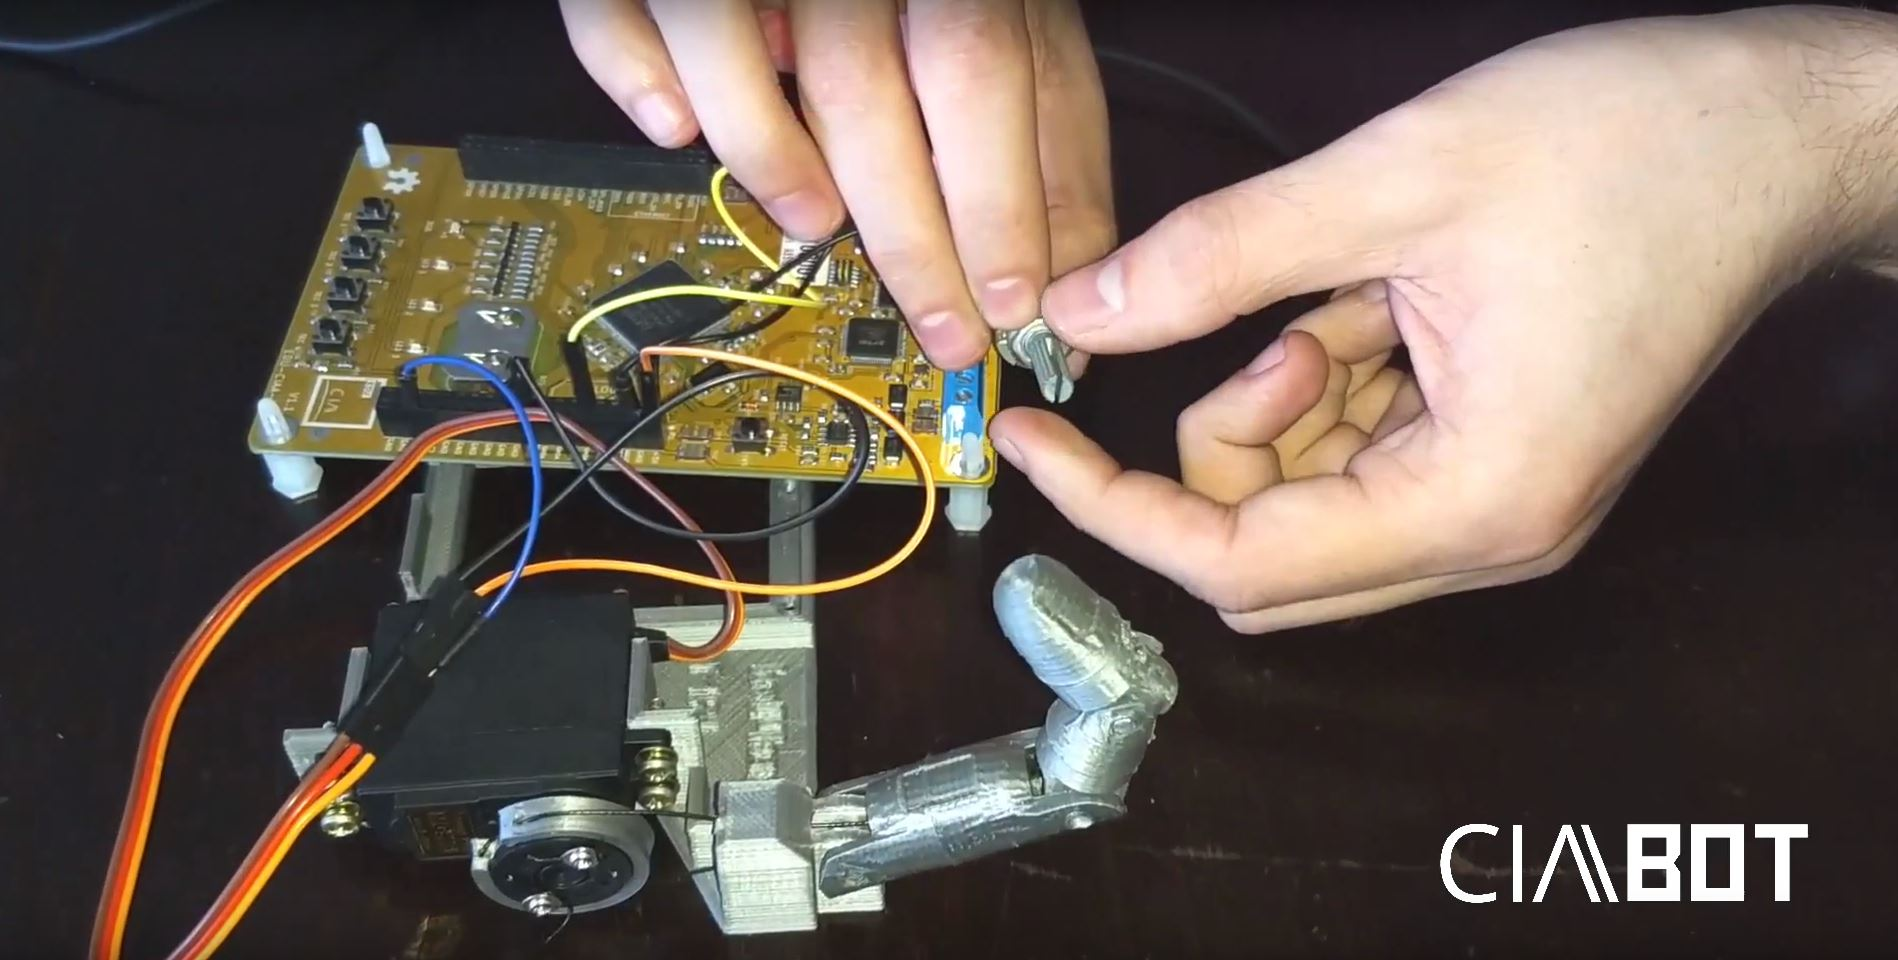
\includegraphics[scale=.3]{./Figures/dedo-servo.jpg}
\caption{Prueba de servomotor sobre dedo 3D.}
\label{fig:dedoServo}
\end{figure}

Teniendo en mente la necesidad de desarrollar ejemplos didácticos para utilizar CIAABOT, se utilizaron materiales desarrollados y provistos por la Universidad Nacional de Quilmes, en el marco del proyecto "La universidad y la escuela secundaria", dirigido por Cristina Wainmaier (Vicedirectora del Dto. de CyT, UNQ). Estos materiales incluían una maqueta de manejo de barreras y semáforos e instrumentos meteorológicos.

Para la verificación del correcto manejo del tiempo por parte del programa, se utilizó un anemómetro. Este dispositivo, que puede apreciarse en la figura \ref{fig:anemometro}, gira ante la presencia de viento y genera pulsos a intervalos angulares fijos. Conociendo la frecuencia de estos pulsos es posible determinar la velocidad del viento en cada momento.

Además, en este ensayo se probó la UART, proveyendo de una salida de consola por puerto serie, que podía observarse desde la PC. De esta manera el programa podía informar las mediciones realizadas, y guardarse en un archivo de log.

\begin{figure}[h]
\centering
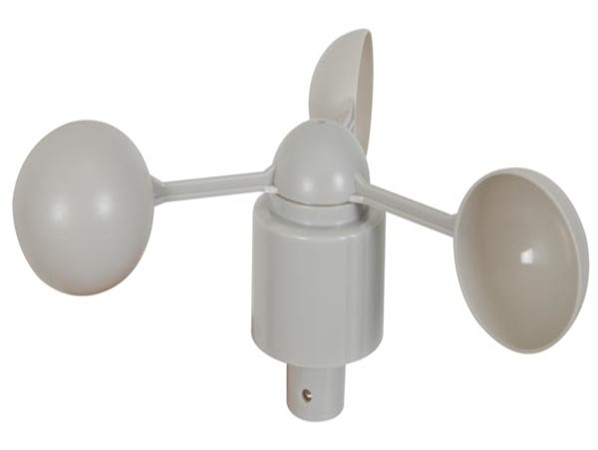
\includegraphics[scale=.8]{./Figures/anemometro.jpg}
\caption{Anemómetro utilizado en las pruebas.}
\label{fig:anemometro}
\end{figure}

De los instrumentos meteorológicos también se utilizó una rosa de los vientos formada por una matriz de leds. Con esto se validó el funcionamiento de las salidas digitales funcionando a la vez. En la figura \ref{fig:rosaVientos}, se observa un dibujo de la rosa de los vientos utilizada, así como la conexión de la matriz de leds que posee para encender los diferentes puntos cardinales.

\begin{figure}[H]
\centering
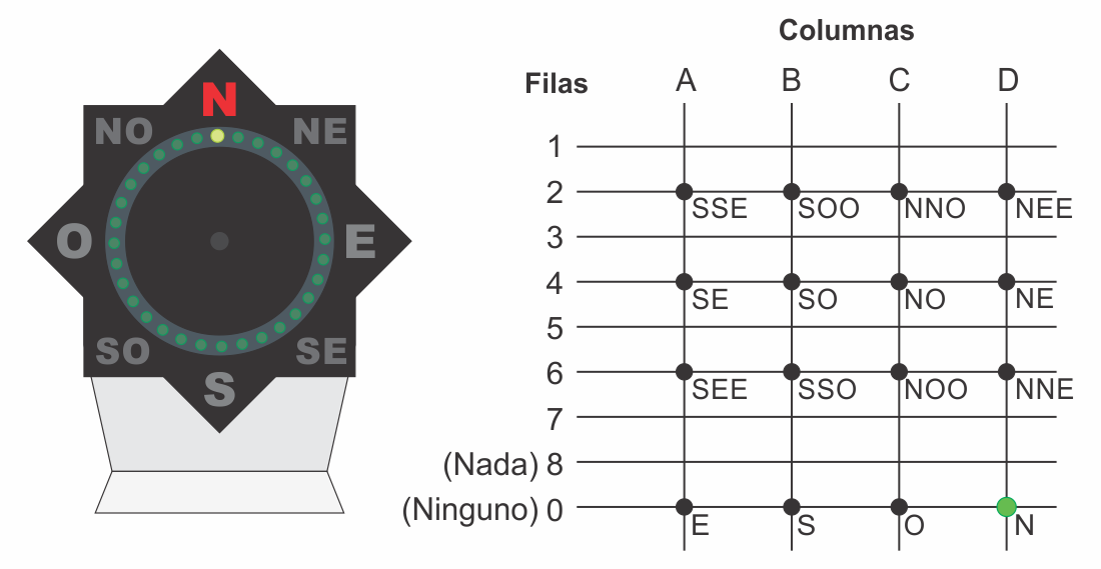
\includegraphics[scale=.6]{./Figures/rosa-vientos.png}
\caption{Rosa de los vientos y conexión de los leds.}
\label{fig:rosaVientos}
\end{figure}

\section{Workshop en el SASE}
Desde el 2010 se viene realizando año a año el Simposio Argentino de Sistemas Embebidos. Este evento es organizado por ACSE (Asociación Civil para la Investigación Promoción y Desarrollo de los Sistemas Electrónicos Embebidos). Es un evento anual que reúne a la comunidad académica y a la industria  en torno a esta temática, donde se realizan Tutoriales, Workshops y el Congreso Argentino de Sistemas Embebidos. 

En la edición de este año se agregó el workshop "Introducción a la programación de sistemas embebidos utilizando CIAABOT", que tuve la posibilidad de dictar y organizar en conjunto con el Ing. Eric Pernía. Estuvo orientado principalmente a alumnos de escuelas secundarias o entusiastas que buscaran una introducción a la programación de embebidos pero que no tuvieran conocimientos de ningún lenguaje para hacerlo.

Con una buena concurrencia se desarrolló la primera experiencia real en campo de la utilización de la plataforma CIAABOT para la enseñanza de programación. Se abarcaron temas básicos como el funcionamiento de sentencias condicionales, estructuras de control, lógica booleana y manejo básico de periféricos.

El workshop se realizó utilizando solamente CIAABOT IDE como medio para programar las placas. Se hizo uso de los elementos meteorológicos y la maqueta vehicular descrita en la sección \ref{sec:pruebas}, que puede observarse en la figura \ref{fig:maqueta}. Fue una buena oportunidad para obtener devoluciones por parte de los primeros usuarios de prueba, que fueron los asistentes al curso. Encontraron la aplicación intuitiva y se desenvolvieron de manera natural. Hubo dos casos puntuales de personas que no habían programado nunca antes de asistir, y ambos pudieron completar satisfactoriamente los ejercicios propuestos.

\begin{figure}[H]
\centering
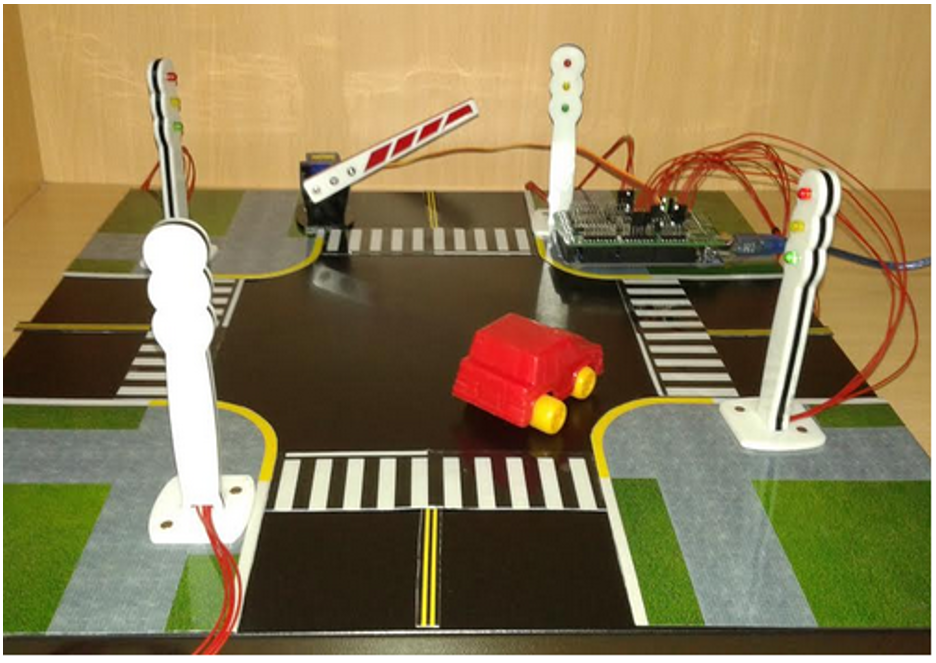
\includegraphics[scale=.8]{./Figures/maqueta.png}
\caption{Maqueta vehicular utilizada en el workshop.}
\label{fig:maqueta}
\end{figure}

\section{Experiencias en cursos CAPSE y de INET}
Los Cursos Abiertos de Programación de Sistemas Embebidos están orientados a personas con o sin experiencia previa, como docentes secundarios o universitarios, personal de empresas o estudiantes, que estén interesados en aprender a trabajar con sistemas embebidos. El objetivo de los cursos es aprender a realizar aplicaciones electrónicoas basadas en microcontroladores ARM de 32 bits, abordando desde problemas simples hasta problemas de mayor complejidad. Se utilizan kits compuestos por sensores y actuadores, y placas EDU-CIAA-NXP.

Además, cursos similares, y con objetivos alineados a los de los CAPSE, se brindaron a pedido del Instituto Nacional de Educación Tecnológica (INET).

En la última edición de estos cursos se utilizó CIAABOT IDE para las primeras clases, como manera de introducir a los asistentes a los conceptos básicos de la programación, así como también para obtener resultados rápidos. 

Esta segunda experiencia de uso de CIAABOT en un entorno real de enseñanza fue realmente útil. Se obtuvieron recomendaciones y se registraron errores descubiertos a raíz de casos de uso que no se tuvieron en cuenta a la hora del desarrollo. Todas estas mejoras y errores fueron registrados en la sección de \emph{issues} del repositorio de CIAABOT.

Por ejemplo, gran parte de los asistentes poseían netbooks con pantallas de resolución limitada, lo que hacía algo dificultoso el manejo de la vista partida que presenta el editor gráfico del IDE en conjunto con la salida del código C. Además, la sección de proyectos recientes y el formulario de 'Nuevo Proyecto' no se mostraban de manera cómoda. A raíz de esto, se comenzó un proceso de mejora de la adaptación de la aplicación ante cambios de resoluciones de pantalla, a lo que se refiere en inglés como  \emph{responsiveness}.

\section{Uso en un proyecto de brazo robótico}
El Laboratorio Abierto de la Universidad Tecnológica Nacional Facultad Regional Avellaneda, comenzó este año el desarrollo de una prótesis de brazo y mano robótica, impresas en 3D. La mano cuenta con movilidad en la muñeca y las falanges de los dedos, logrando así una funcionalidad similar a la de la mano humana. El brazo puede observarse en la figura \ref{fig:brazo}.

\begin{figure}[H]
\centering
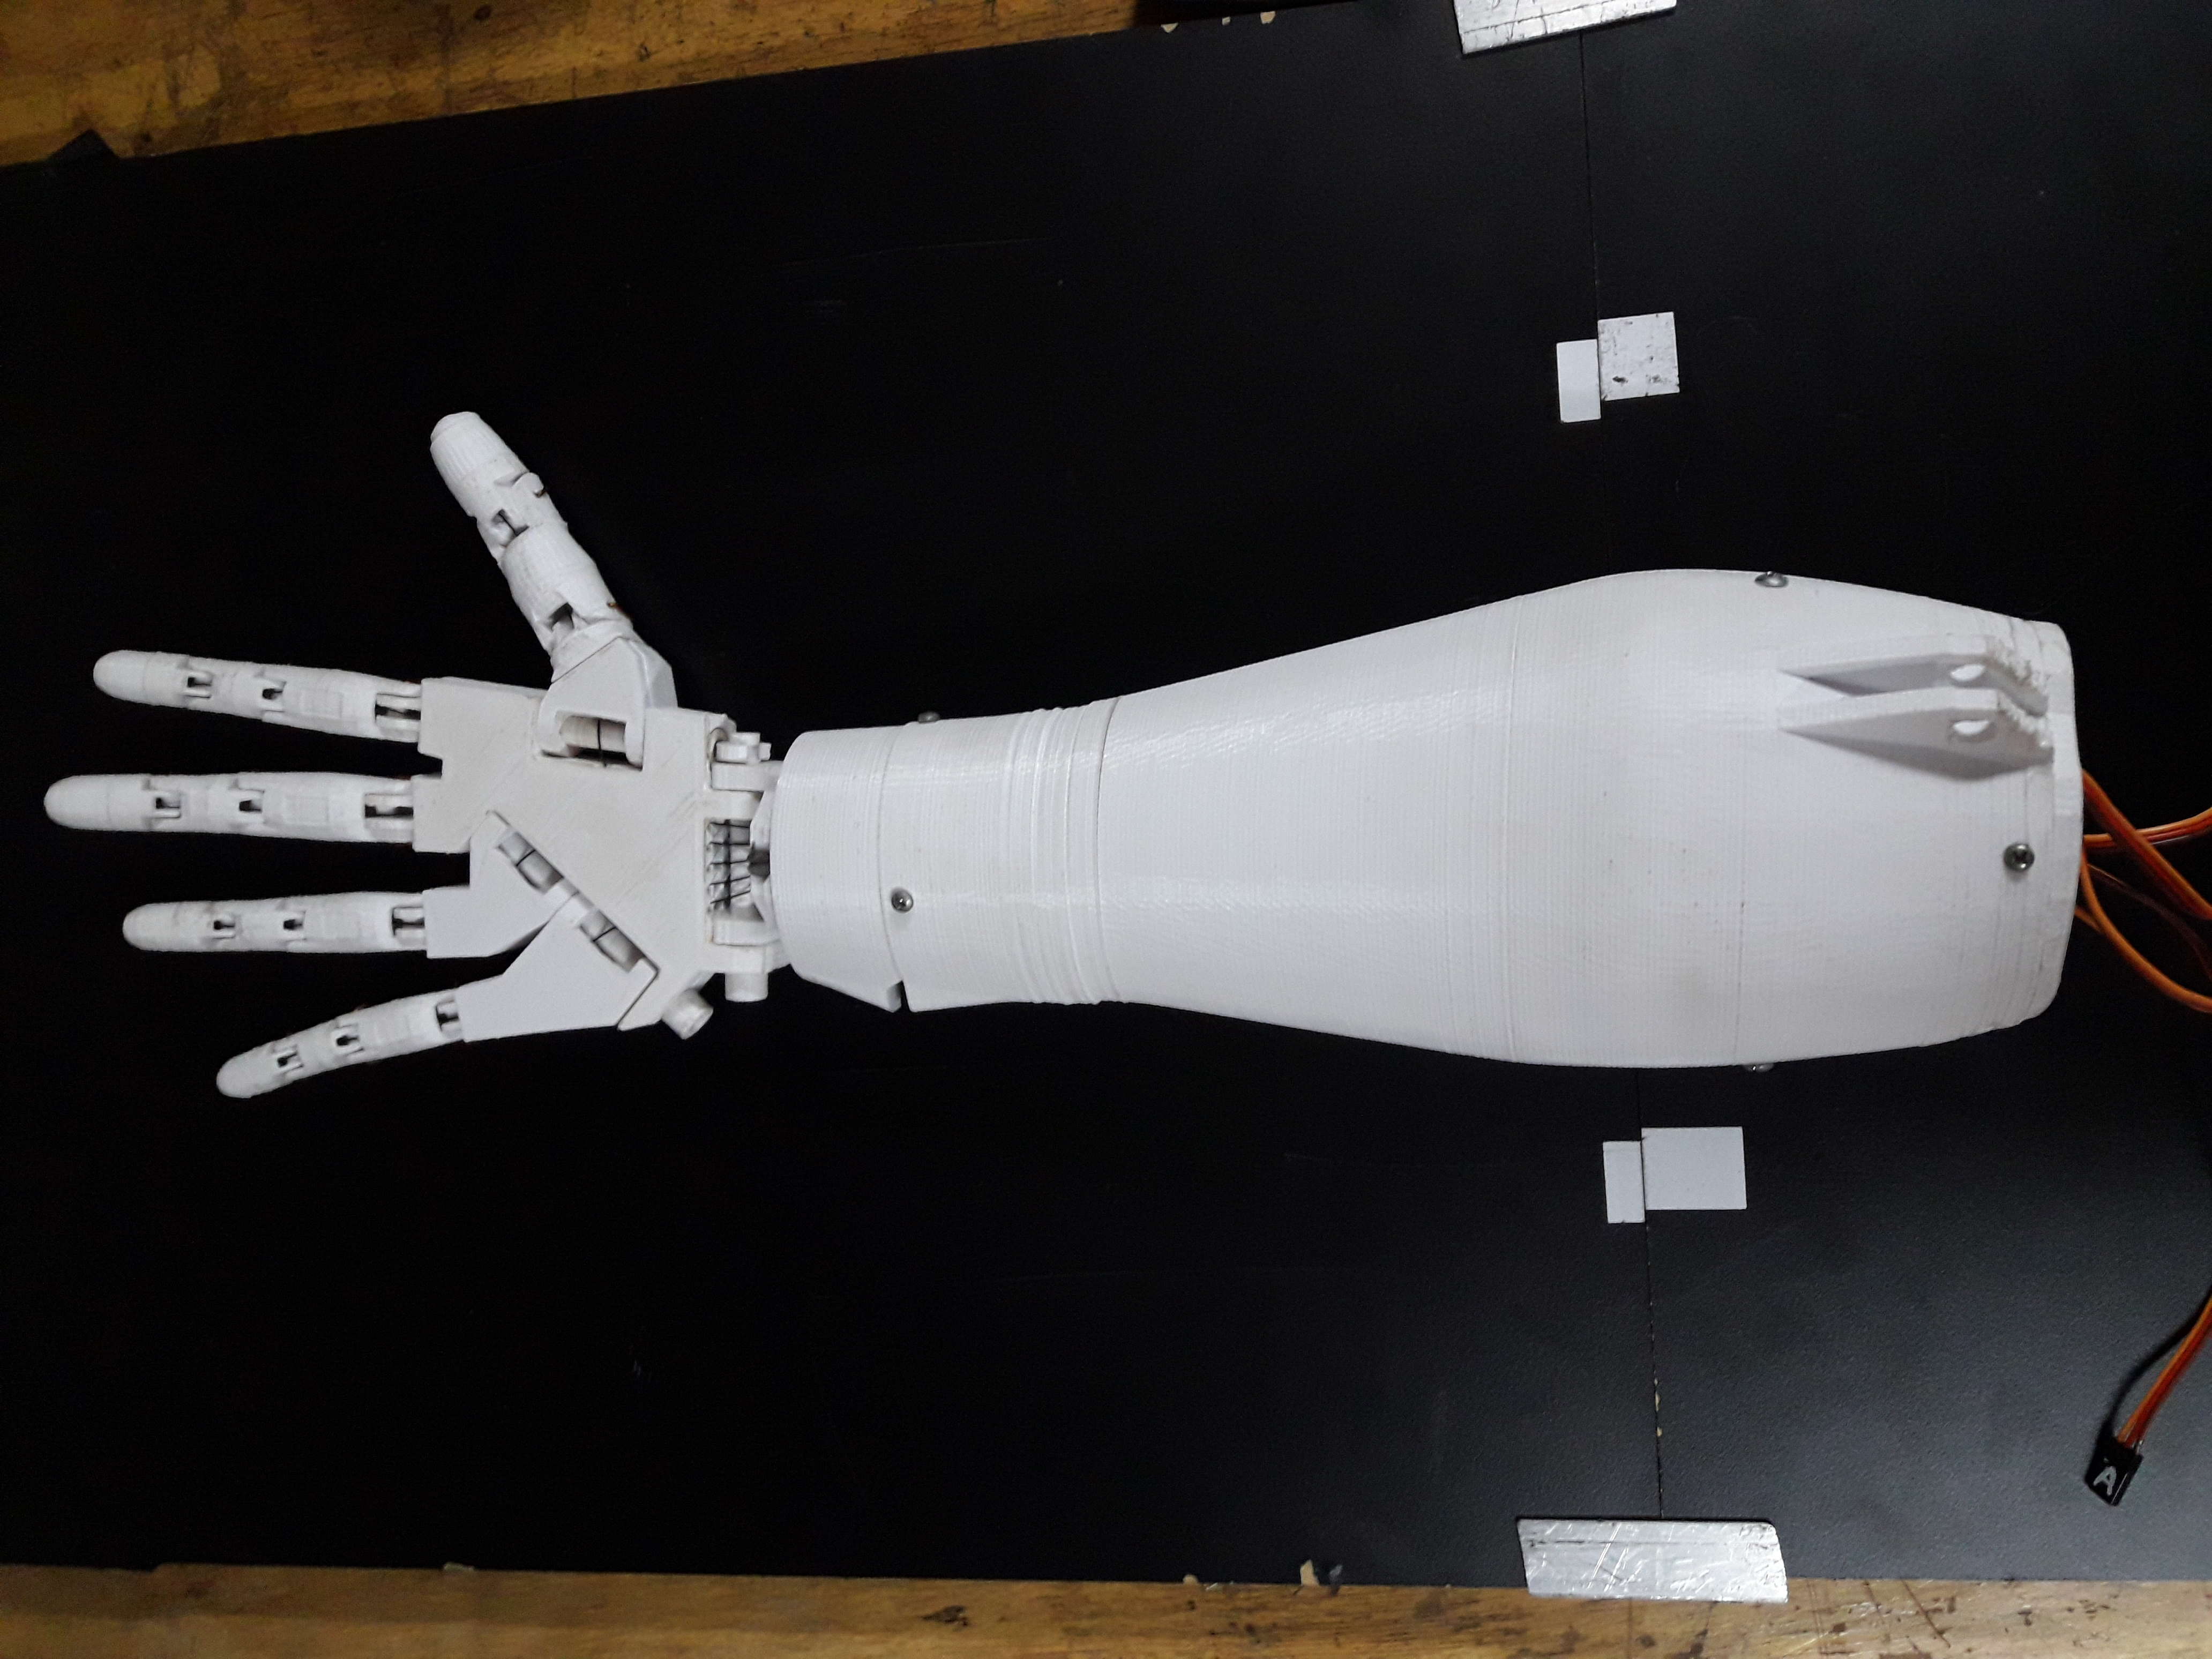
\includegraphics[scale=.1]{./Figures/brazo.jpg}
\caption{Prótesis impresa en 3D.}
\label{fig:brazo}
\end{figure}

El objetivo principal del mismo, es poder realizar un aporte a la mejora de la calidad de vida de personas con amputaciones parciales de brazo y mano. Se utilizan las señales bioeléctricas obtenidas superficialmente desde el músculo del usuario para luego transformarla en una señal eléctrica capaz de manipularse, con el fin de controlarla. Por tal motivo, el faltante de miembro del paciente no debe ser total, para permitir una colocación de 3 electrodos.

Actualmente el proyecto busca migrarse a microcontroladores de 32 bits, y se optó utilizar la placa EDU-CIAA-NXP. Esto es debido a que las mediciones de los electrodos sirven para realizar un control rudimentario y detectar si el músculo está contraído o no, pero no alcanza para obtener una señal proporcional a la fuerza ejercida para emular este movimiento en la prótesis.

La idea es mejorar algoritmo de detección de fuerza en el músculo, realizando un análisis en el dominio de la frecuencia con el objetivo de eliminar ruidos propios que se generan por el tipo de contacto que tienen los sensores. Para esto, se pretende hacer uso de la unidad de punto flotante presente en el LPC4337. Para las primeras pruebas de manejo de hardware y lectura de los sensores musculares, se utilizaron programas armados en CIAABOT IDE.
